\documentclass{article}
\usepackage{tikz}
\usepackage{amsmath}
\usetikzlibrary{external}
\tikzexternalize

\newcommand{\Err}{E}

\begin{document}

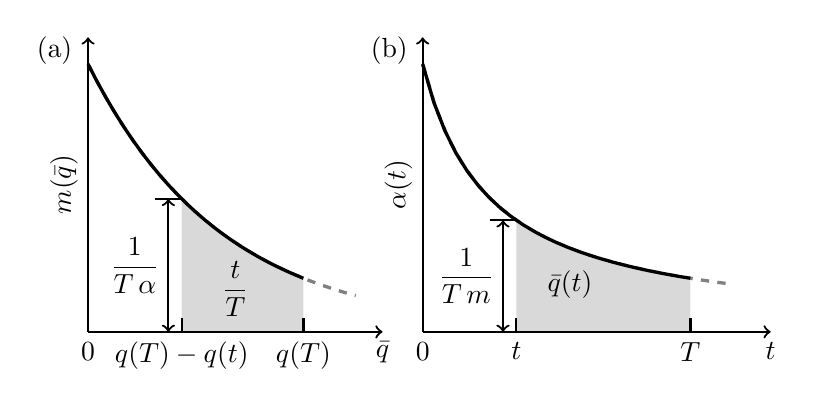
\begin{tikzpicture}[thick, scale=1.7, every node/.style={scale=1.0}]
  \begin{scope}[shift={(0,0)}]
    \node [] at (-0.25, 2.1) {(a)};

    % distribution
    \draw[domain=0:2.0, variable=\x, dashed, gray, very thick]
      plot({\x}, {2*exp(-\x)});

    % shade
    \fill [gray!30!white, domain=0.7:1.609, variable=\x]
      (0.7, 0) --
      plot ({\x}, {2*exp(-\x)})
      -- (1.609, 0) -- cycle;

    % thick curve
    \draw[domain=0:1.609, variable=\x, very thick]
      plot({\x}, {2*exp(-\x)});

    % label for the shaded area
    \node[] at (1.1, 0.32) {$\dfrac{t}{T}$};

    \draw[<->] (0.6, 0)  --
               node[left, inner sep=1mm]
               {$\dfrac{1}{T \, \alpha}$}
               (0.6, 0.99317);
    % label for the ordinate
    %\node[fill=white] at (0.4, 0.7) {$\dfrac{1}{Ta}$};

    \draw[] (0.5, 0.99317) -- (0.7, 0.99317);
    \draw[->] (0, 0) -- (2.2, 0);
    \node[] at (2.2, -0.15) {$\bar q$};
    \draw[->] (0, 0) -- node[above, rotate=90] {$m(\bar q)$} (0, 2.2);

    % xtics
    \draw[] (0.0, 0.1) -- (0.0, 0.0) node[below] {$0$};
    \draw[] (0.7, 0.1) -- (0.7, 0.0) node[below] {$q(T) - q(t)$};
    \draw[] (1.609, 0.1) -- (1.609, 0.0) node[below] {$q(T)$};
  \end{scope}

  \begin{scope}[shift={(2.5,0)}]
    \node [] at (-0.25, 2.1) {(b)};
    % distribution
    \draw[domain=0:2.3, variable=\x, dashed, gray, very thick]
      plot({\x}, {1/(\x+0.5)});

    % shade
    \fill [gray!30!white, domain=0.7:2.0, variable=\x]
      (0.7, 0) --
      plot ({\x}, {1/(\x+0.5)})
      -- (2.0, 0) -- cycle;

    % thick curve
    \draw[domain=0:2.0, variable=\x, very thick]
      plot({\x}, {1/(\x+0.5)});

    % label for the shaded area
    \node[] at (1.1, 0.35) {$\bar q(t)$};

    \draw[<->] (0.6, 0)  --
               node[left, inner sep=1mm]
               {$\dfrac{1}{T \, m}$}
               (0.6, 0.83333);
    % label for the ordinate
    %\node[fill=white] at (0.4, 0.7) {$\dfrac{1}{Ta}$};

    \draw[] (0.5, 0.83333) -- (0.7, 0.83333);
    \draw[->] (0, 0) -- (2.6, 0);
    \node[] at (2.6, -0.14) {$t$};
    \draw[->] (0, 0) -- node[above, rotate=90] {$\alpha(t)$} (0, 2.2);

    % xtics
    \draw[] (0.0, 0.1) -- (0.0, 0.0) node[below] {$0$};
    \draw[] (0.7, 0.1) -- (0.7, 0.0) node[below] {$t$};
    \draw[] (2.0, 0.1) -- (2.0, 0.0) node[below] {$T$};
  \end{scope}
\end{tikzpicture}


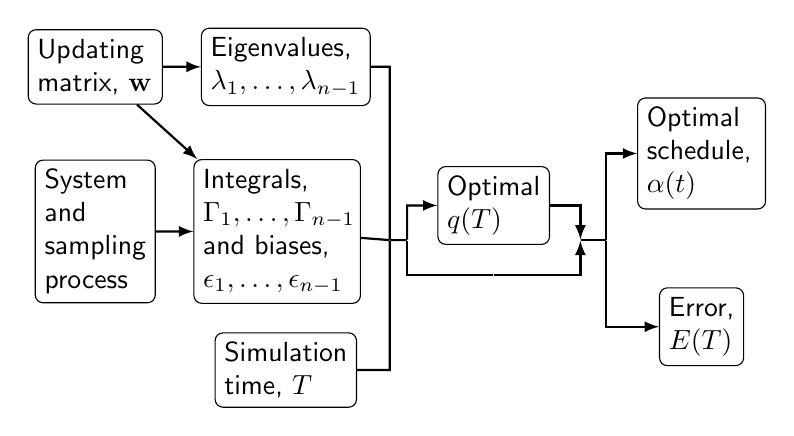
\begin{tikzpicture}[scale=1.1, every node/.style={rounded corners=0.1cm}]\sffamily
  \node[draw, text width={width("Updating ")}]
    (w) at (0, 3) {Updating \\matrix, $\mathbf w$};

  \node[draw, text width={width("sampling")}]
    (sys) at (0, 1.1) {System\\and\\sampling\\process};

  \node[draw, text width={width("Eigenvalues, ")}]
    (lambda) at (2.2, 3) {Eigenvalues,\\$\lambda_1, \dots, \lambda_{n-1}$};

  \node[draw, text width={width("Integrals, iiiii")}]
    (Gamma) at (2.1, 1.1) {Integrals, \\$\Gamma_1, \dots, \Gamma_{n-1}$\\and biases,\\$\epsilon_1, \dots, \epsilon_{n-1}$};

  \node[draw, text width={width("Simulation")}]
    (T) at (2.2, -0.5) {Simulation\\time, $T$};

  \node[draw, text width={width("Optimal")}]
    (qT) at (4.6, 1.4) {Optimal\\ $q(T)$};

  \node[draw, text width={width("Schedule,")}]
    (alpha) at (7, 2) {Optimal schedule,\\ $\alpha(t)$};

    \node[draw, text width={width("Error,")}]
    (err) at (7, 0) {Error, $\Err(T)$};

  \node[inner sep=0, minimum size=0] (M1) at (3.4, 1) {};

  \node[inner sep=0, minimum size=0] (N1) at (5.9, 1) {};

  \node[inner sep=0, minimum size=0] (R1) at (3.6, 1) {};
  \node[inner sep=0, minimum size=0] (R2) at (4.6, 0.6) {};
  \node[inner sep=0, minimum size=0] (R3) at (5.6, 1) {};

  \draw[->, >=latex, thick]
    (w) edge (lambda)
    (w) edge (Gamma)
    (sys) edge (Gamma);

  \draw[->, >=latex, thick]
    (lambda) -| (M1)
    (Gamma)  -- (M1)
    (T)      -| (M1)
    (M1)     -- (R1)
    (R1)     |- (qT);

  \draw[->, >=latex, thick]
    (qT)     -| (R3);

  \draw[->, >=latex, thick]
    (R3) -- (N1) |- (alpha);

  \draw[->, >=latex, thick]
    (N1) |- (err);

  \draw[->, >=latex, thick]
    %(M1) edge[bend left=70] (N1);
    (R1) |- (R2) -| (R3);
\end{tikzpicture}

\end{document}
